\documentclass{article}
\usepackage[utf8]{inputenc}
\usepackage[T1]{fontenc}
\usepackage[russian]{babel}
\usepackage{tikz}
\usepackage{graphicx}
\usepackage{titlesec}
\usepackage{amsfonts}
\usepackage{amsmath}
\usepackage{bbm}
\usepackage[left=2cm,right=2cm,
    top=2cm,bottom=2cm,bindingoffset=0cm]{geometry}
\renewcommand{\thesection}{\arabic{section}}
\titleformat{\section}{\large\bfseries}{\thesection}{1em}{}
\title{Пределы}
\author{Каренин Константин Витальевич}
\date{9.11.2023}
\begin{document}

\begin{titlepage}
    \centering
    \vspace*{0.5 cm}
    
    \textsc{\LARGE \textbf{Линейная алгебра}}
    \vspace{1.5cm}
    
    \rule{\linewidth}{0.2 mm} \\[0.4 cm]
    { \huge \bfseries Линейная алгебра}
    \rule{\linewidth}{0.2 mm} \\[1.5 cm]
    
    \Large Выполнили: \\
    Каренин Константин \\
    Темиров Тимур \\
    Гонин Сергей \\
    
    \vspace{0.5cm}
    
    Группа: М3104
    
    \vspace{0.5cm}
    
    Преподаватель: Сарычев Павел
    
    \vspace{0.5cm}
    
    Университет ИТМО
    
    \vfill

    
\includegraphics[height=70px]{logo.jpg}
    
    9.11.2023
    
\end{titlepage}

\setcounter{page}{2}

% task 1
\newpage
    \section{Задание 1}
    \[
    A = \begin{pmatrix}
        1 & -2 & 1 \\
        2 & 3 & -1 \\
        4 & -1 & 1 \\
    \end{pmatrix}
    ,
    B = \begin{pmatrix}
        4 \\
        3 \\
        11 \\
    \end{pmatrix}
    \]
   
   \subsection{Решение подзадания 1}
   
    \[
    \begin{pmatrix}
        1 & -2 & 1 \\
        2 & 3 & -1 \\
        4 & -1 & 1 \\
    \end{pmatrix}X=0 \\
    \]
    \[
    \begin{pmatrix}
        1 & -2 & 1 \\
        2 & 3 & -1 \\
        4 & -1 & 1 \\
    \end{pmatrix} 
    \to
    \begin{pmatrix}
        1 &	-2 & 1 \\
        0 & 7 & -3 \\
        4 & -1 & 1 \\
    \end{pmatrix}
    \to
    \begin{pmatrix}
        1 &	-2 & 1 \\
        0 & 7 & -3 \\
        0 & 7 & -3 \\
    \end{pmatrix}
    \to
    \begin{pmatrix}
        1 &	-2 & 1 \\
        0 & 0 & 0 \\
        0 & 7 & -3 \\
    \end{pmatrix} \\ \\ 
    \]
    Возьмем $x_2$ как свободную переменную, тогда \\ \\
    $x_1 = -\frac{1}{3}x_2$ \\ \\
    $x_3 = \frac{7}{3}x_2$ \\ \\
    Пусть $x_2 = 3$, тогда \\ \\
    $x_1 = -x_2$ \\ \\
    $x_3 = 7x_2$ \\ \\
    Получился базис $\delta = 
    \begin{pmatrix}
        -1 \\
        3 \\
        7\\
    \end{pmatrix}$, который образует одномерное линейное пространство: \\ \\
    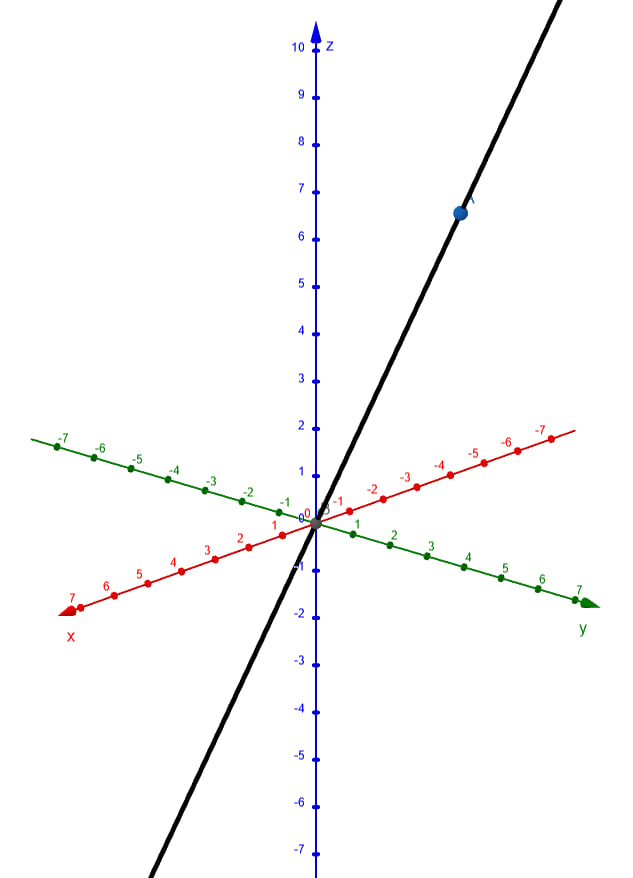
\includegraphics[height=200px]{1.1.jpg} \\ \\ \\ \\ \\ \\ \\ \\ \\ \\ \\
    Проекции: \\
    На плоскость $xy$: \\
    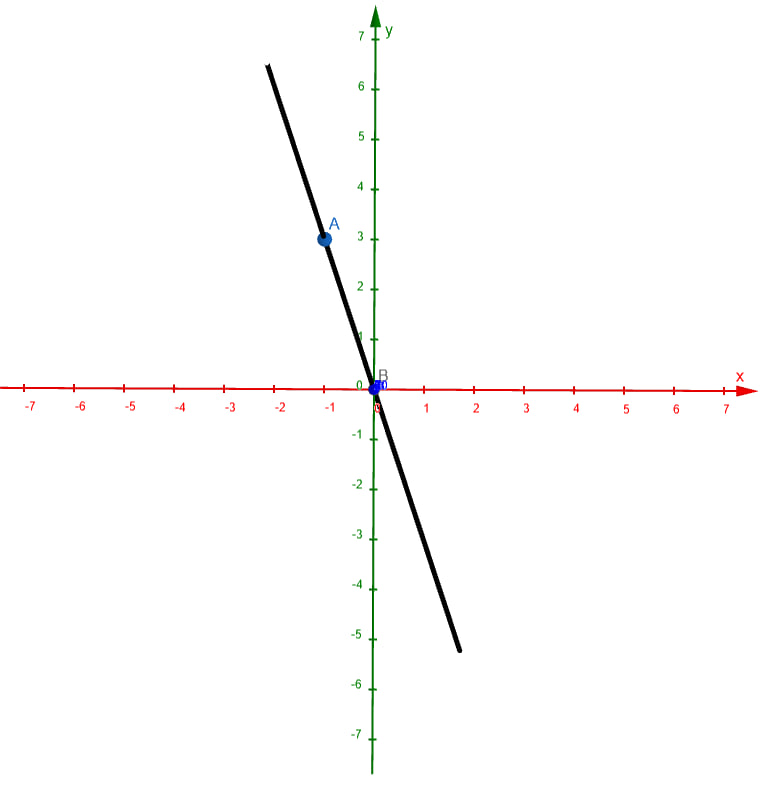
\includegraphics[height=200px]{1.xy.jpg} \\
    На плоскость $xz$: \\
    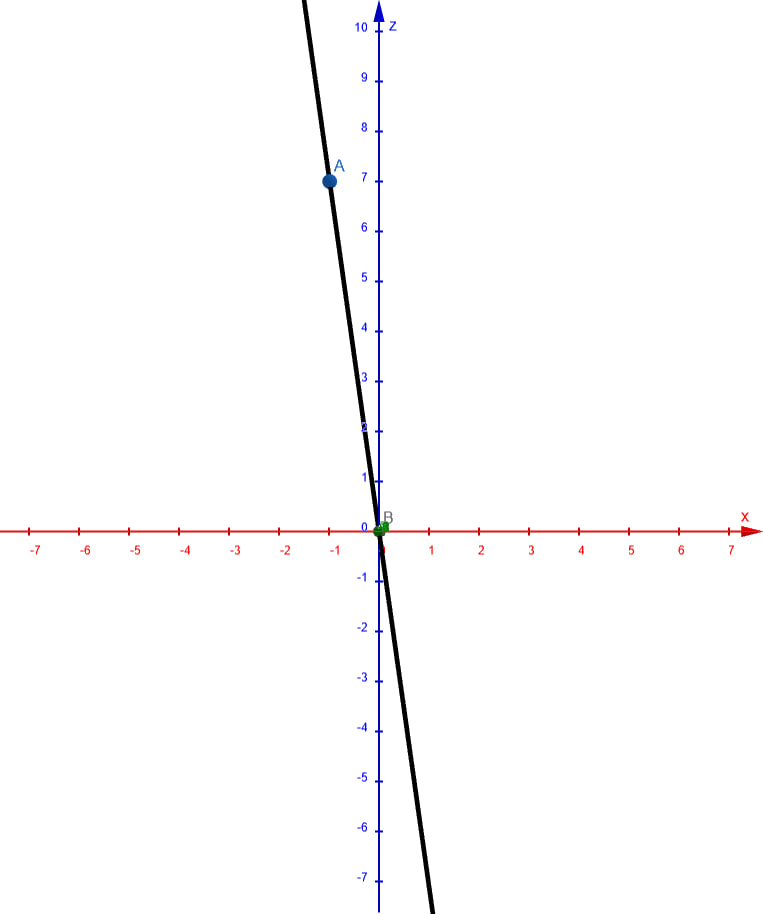
\includegraphics[height=200px]{1.xz.jpg} \\
    На плоскость $yz$: \\
    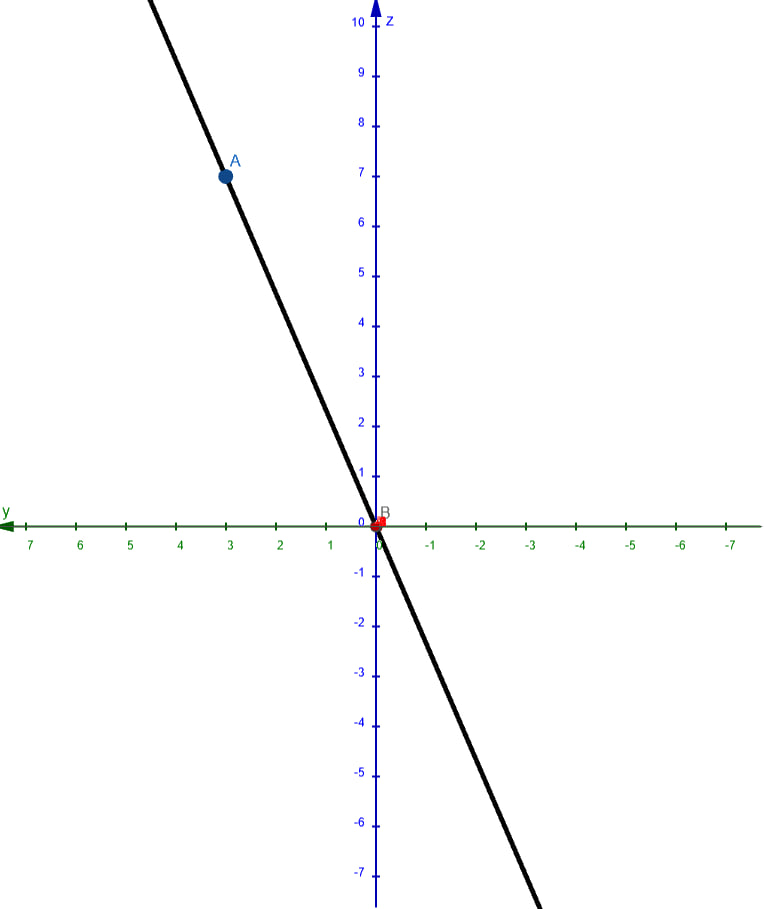
\includegraphics[height=200px]{1.yz.jpg} \\

    \subsection{Решение подзадания 2}
    \subsubsection{Совместность}
    Система $AX = B$ совместна \iff $rank(A) = rank(A|B)$ \\
    $rank(A) = 2$ \\ \\
    \[A|B = 
    \begin{pmatrix}  
        1 &	-2 & 1 & | & 4 \\ 
        2 &	3 &	-1 & | & 3 \\
        4 &	-1 & 1 & | & 11 \\
    \end{pmatrix}
    \to
    \begin{pmatrix}  
        1 &	-2 & 1 & | & 4 \\ 
        0 &	7 &	-3 & | & 5 \\
        4 &	-1 & 1 & | & 11 \\
    \end{pmatrix}
    \to
    \begin{pmatrix}  
        1 &	-2 & 1 & | & 4 \\ 
        0 &	7 &	-3 & | & -5 \\
        0 &	7 & -3 & | & -5 \\
    \end{pmatrix}
    \to
    \begin{pmatrix}  
        1 &	-2 & 1 & | & 4 \\ 
        0 &	7 &	-3 & | & -5 \\
        0 &	0 & 0 & | & 0 \\
    \end{pmatrix} \\ \\ \\
    \] 
    $rank(A|B) = 2$ \\
    $rank(A) = rank(A|B) \Rightarrow$ система совместна
    \subsubsection{Неопределённость}
    Система $AX = B$ неопределённая \iff $система имеет больше одного решения$ \\ \\
    \[
    \begin{pmatrix}  
        1 &	-2 & 1 & | & 4 \\ 
        2 &	3 &	-1 & | & 3 \\
        4 &	-1 & 1 & | & 11 \\
    \end{pmatrix}
    \to
    \begin{pmatrix}  
        1 &	-2 & 1 & | & 4 \\ 
        0 &	7 &	-3 & | & 5 \\
        4 &	-1 & 1 & | & 11 \\
    \end{pmatrix}
    \to
    \begin{pmatrix}  
        1 &	-2 & 1 & | & 4 \\ 
        0 &	7 &	-3 & | & -5 \\
        0 &	7 & -3 & | & -5 \\
    \end{pmatrix}
    \to
    \begin{pmatrix}  
        1 &	-2 & 1 & | & 4 \\
        0 &	0 & 0 & | & 0 \\
        0 &	7 &	-3 & | & -5 \\
    \end{pmatrix} \\ \\ \\
    \] 
    Возьмем $x_2$ как свободную переменную равную $\alpha \in \mathbb{R}$ и получим: \\ \\
    $x_1 = \frac{7}{3}-\frac{1}{3}\alpha$ \\ \\
    $x_2 = \alpha$ \\ \\
    $x_3 = \frac{5}{3} + \frac{7}{3}\alpha$ \\ \\
    Решений получилось больше одного $\Rightarrow$ система неопределённая \\
    Покажем множество решений на том же графике: \\ \\
    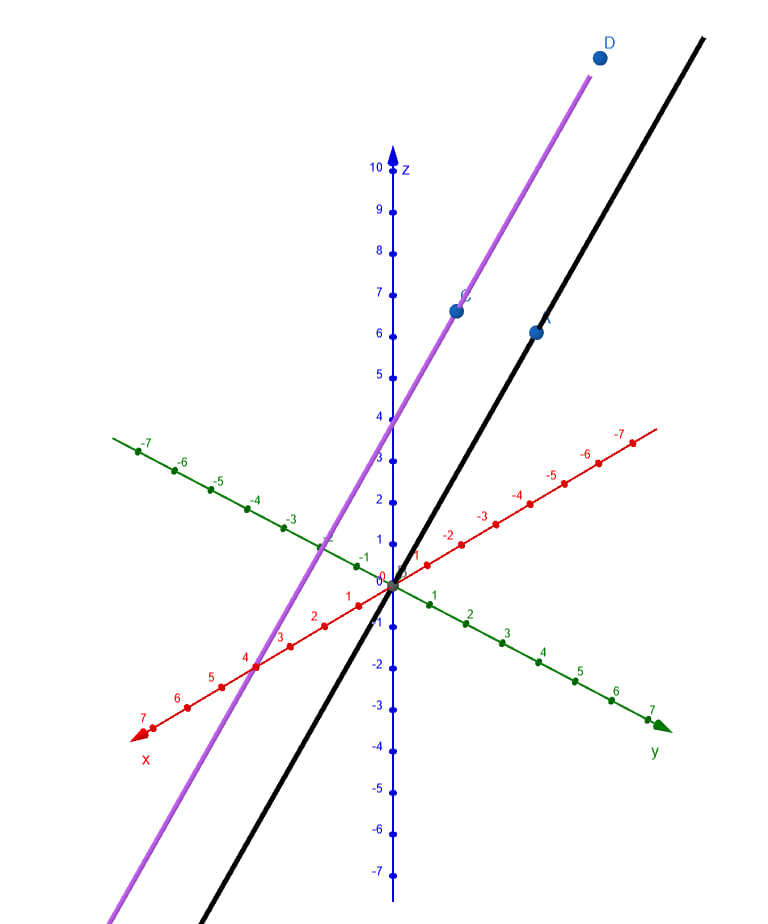
\includegraphics[height=200px]{2.1.jpg} \\ \\ \\ \\ \\ \\ \\ \\
    Проекции: \\
    На плоскость $xy$: \\
    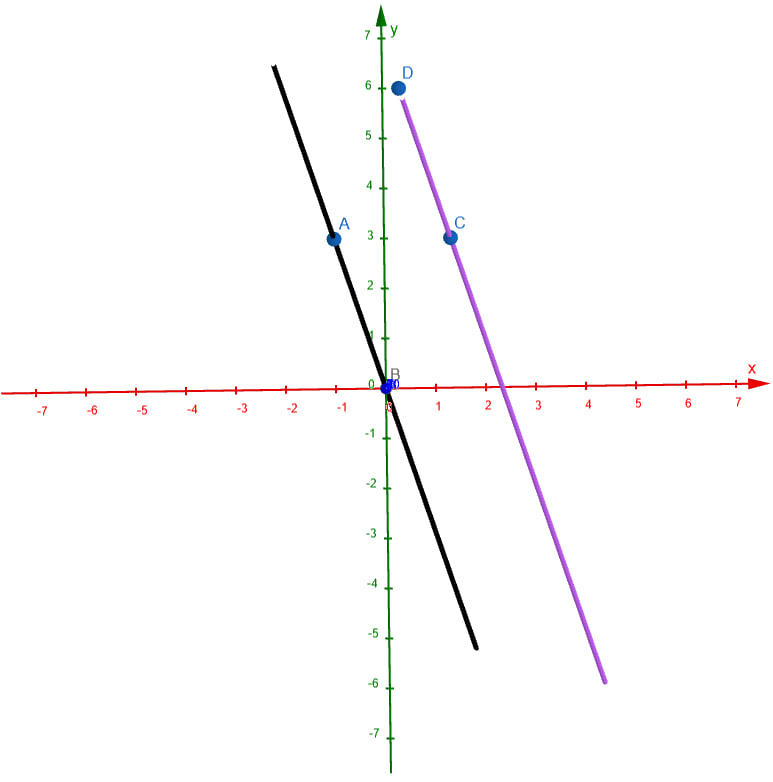
\includegraphics[height=200px]{2.xy.jpg} \\
    На плоскость $xz$: \\
    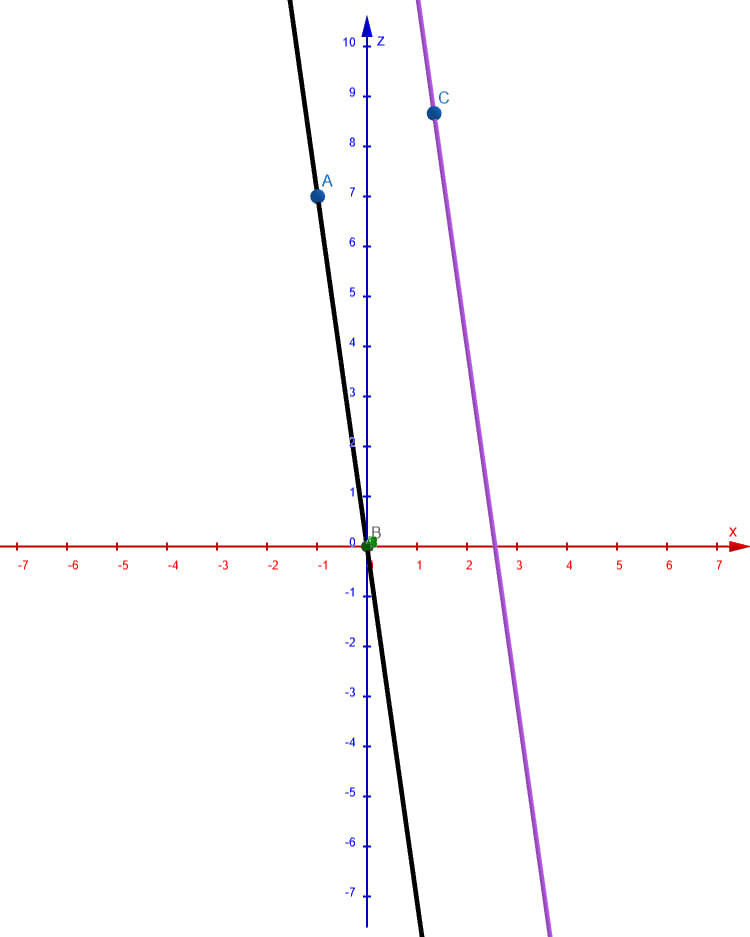
\includegraphics[height=200px]{2xz.jpg} \\
    На плоскость $yz$: \\
    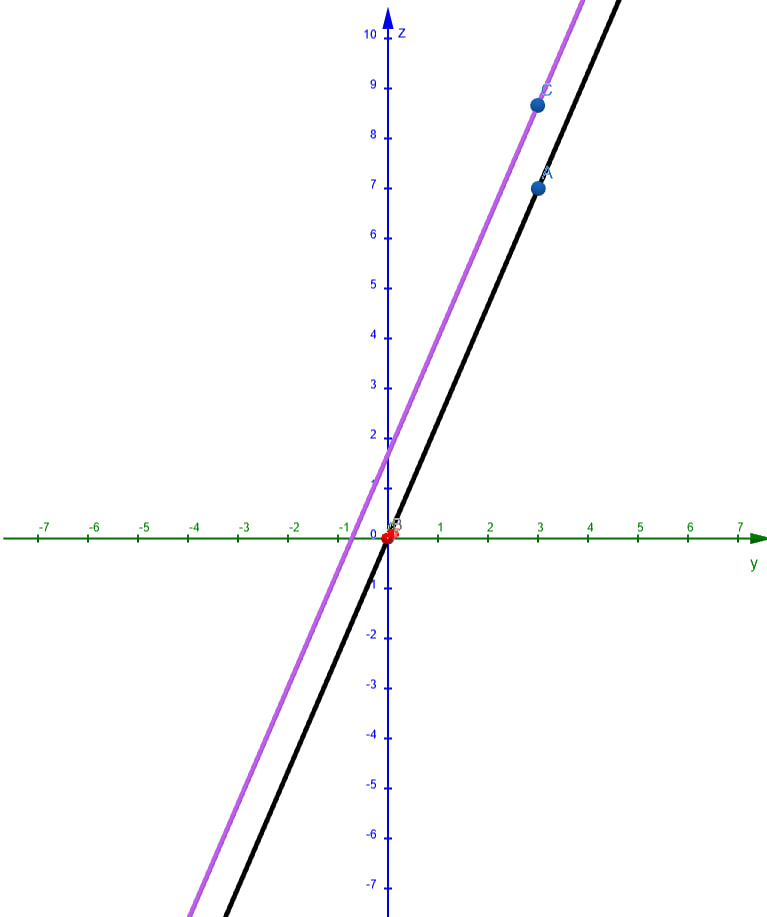
\includegraphics[height=200px]{2.yz.jpg} \\
    
    
    

    
% task 2
\newpage
    \section{Задание 2}
    \[
    A_1 =
    \begin{pmatrix}
        1 & 1 \\
        1 & 1 \\
    \end{pmatrix},
    A_2 =
    \begin{pmatrix}
        1 & -1 \\
        1 & -1 \\
    \end{pmatrix},
    A_3 =
    \begin{pmatrix}
        -1 & 0 \\
        1 & 0 \\
    \end{pmatrix},
    A_4 =
    \begin{pmatrix}
        0 & 1 \\
        0 & -1 \\
    \end{pmatrix},
    x =
    \begin{pmatrix}
        1 & 2 \\
        3 & 4 \\
    \end{pmatrix}
    \]
    \[
    e_1 = 1, e_2 = 1 + t, e_3 = 1 + t + t^2, e_4 = 1 + t + t^2 + t^3, e_4 = 1 + t + t^2 + t^3 + t^4  
    \]

    \subsection{Решение подзадания 1}
    \subsubsection{Доказательство}
    $L - $ линейное пространство матриц второго порядка \\
    $\mathcal{A} \subset L$ \\
    $\mathcal{A} = \{A_1, A_2, A_3, A_4 \}$

    \[
    \mathcal{A} - \text{базис } L \iff 
    \begin{cases}
        \mathcal{A} \subset L \\
        \mathcal{A} \text{ - линейно независимая} \\
        \mathcal{A} \cup \{l_i\} \text{ - линейно зависимый}, l_1 \in L
    \end{cases}
    \]
    1) $\mathcal{A} \subset L$ - по условию \\
    2) Докажем, что $\mathcal{A} \text{ - линейно независимая}$: \\
    $\forall \lambda_i \in \mathbb{R}$ \\
    \mathcal{A} - линейно независимая \iff $\sum\limits_{i=1}^n \lambda_i a_i = \mathbbm{O} \Rightarrow \forall \lambda_i = \mathbbm{O}$ \\
    \[\lambda_1
    \begin{pmatrix}
        1 & 1 \\
        1 & 1 \\
    \end{pmatrix}
    + \lambda_2
    \begin{pmatrix}
        1 & -1 \\
        1 & -1 \\
    \end{pmatrix}
    + \lambda_3
    \begin{pmatrix}
        -1 & 0 \\
        1 & 0 \\
    \end{pmatrix}
    + \lambda_4
    \begin{pmatrix}
        0 & 1 \\
        0 & -1 \\
    \end{pmatrix}
    = \mathbbm{O}
    \]
    \[
    \begin{pmatrix}
        \lambda_1 + \lambda_2 - \lambda_3 & \lambda_1 - \lambda_2 + \lambda_4 \\
        \lambda_1 + \lambda_2 + \lambda_3 & \lambda_1 - \lambda_2 - \lambda_4 \\
    \end{pmatrix}
    = \mathbbm{O} \Rightarrow
    \]
    \[
    \begin{cases}
        \lambda_1 + \lambda_2 - \lambda_3 = 0 \\
        \lambda_1 - \lambda_2 - \lambda_4 = 0 \\
        \lambda_1 + \lambda_2 + \lambda_3 = 0 \\
        \lambda_1 - \lambda_2 - \lambda_4 = 0 \\
    \end{cases}
    \begin{cases}
        \lambda_1 = \lambda_3 - \lambda_2 \\
        \lambda_3 - 2\lambda_2 + \lambda_4 = 0 \\
        \lambda_3 = 0 \\
        \lambda_3 - 2\lambda_2 - \lambda_4 = 0 \\
    \end{cases}
    \begin{cases}
        \lambda_1 = - \lambda_2 \\
        \lambda_4 = 2\lambda_2 \\
        \lambda_3 = 0 \\
        -4\lambda_2 = 0 \\
    \end{cases}
    \begin{cases}
        \lambda_1 = 0 \\
        \lambda_2 = 0 \\
        \lambda_3 = 0 \\
        \lambda_4 = 0 \\
    \end{cases} \Rightarrow \mathcal{A} \text{ - линейно независимая}
    \]
    3)Докажем, что $\mathcal{A} \cup \{l_i\} \text{ - линейно зависимый}, l_1 \in L$ \iff \exists $\sum\limits_{j=1}^{n-1} \lambda_j a_j = a_k \in \mathcal{A} \cup \{l_i\} \forall a_i \in \mathcal{A} \cup \{l_i\}$ \\
    \[
    \lambda_1
    \begin{pmatrix}
        1 & 1 \\
        1 & 1 \\
    \end{pmatrix}
    + \lambda_2
    \begin{pmatrix}
        1 & -1 \\
        1 & -1 \\
    \end{pmatrix}
    + \lambda_3
    \begin{pmatrix}
        -1 & 0 \\
        1 & 0 \\
    \end{pmatrix}
    + \lambda_4
    \begin{pmatrix}
        0 & 1 \\
        0 & -1 \\
    \end{pmatrix}
    =
    \begin{pmatrix}
        \lambda_1 + \lambda_2 - \lambda_3 & \lambda_1 - \lambda_2 + \lambda_4 \\
        \lambda_1 + \lambda_2 + \lambda_3 & \lambda_1 - \lambda_2 - \lambda_4 \\
    \end{pmatrix}
    = l_1 \in L
    \]
    Пусть $l_1 = \lambda_i a_i$, тогда $\lambda_i a_i =
    \begin{pmatrix}
        \lambda_1 + \lambda_2 - \lambda_3 & \lambda_1 - \lambda_2 + \lambda_4 \\
        \lambda_1 + \lambda_2 + \lambda_3 & \lambda_1 - \lambda_2 - \lambda_4 \\
    \end{pmatrix} \Rightarrow
    $
    $a_i = 
    \begin{pmatrix}
        \frac{\lambda_1 + \lambda_2 - \lambda_3}{\lambda_i} & \frac{\lambda_1 - \lambda_2 + \lambda_4}{\lambda_i} \\
        \frac{\lambda_1 + \lambda_2 + \lambda_3}{\lambda_i} & \frac{\lambda_1 - \lambda_2 - \lambda_4}{\lambda_i} \\
    \end{pmatrix}
    $, значит $a_i \in L$ мы можем найти коэффициент относительно векторов системы $A$ \\
    Значит, $\mathcal{A} - \text{базис } L$ \\
    Q.E.D.
    \subsubsection{Координаты x}
    Не трудно заметить: \\
    $x =
    \begin{pmatrix}
        1 & 2 \\
        3 & 4 \\
    \end{pmatrix}
    = 2,5
    \begin{pmatrix}
        1 & 1 \\
        1 & 1 \\
    \end{pmatrix}
    - 0,5
    \begin{pmatrix}
        1 & -1 \\
        1 & -1 \\
    \end{pmatrix}
    +
    \begin{pmatrix}
        -1 & 0 \\
        1 & 0 \\
    \end{pmatrix}
    -
    \begin{pmatrix}
        0 & -1 \\
        0 & -1 \\
    \end{pmatrix}
    = 2,5 \mathcal{A}_1 -0,5 \mathcal{A}_2 + \mathcal{A}_3 - \mathcal{A}_4
    $

    \subsection{Решение подзадания 2}
    \subsubsection{Доказательство}
    $L - $ пространство многочленов степени не больше четырёх \\
    $\mathcal{A} \subset L$ \\
    $\mathcal{A} = \{e_1, e_2, e_3, e_4, e_5\}$
    \[
    \mathcal{A} - \text{базис } L \iff 
    \begin{cases}
        \mathcal{A} \subset L \\
        \mathcal{A} \text{ - линейно независимая} \\
        \mathcal{A} \cup \{l_i\} \text{ - линейно зависимый}, l_1 \in L
    \end{cases}
    \]
    1) $\mathcal{A} \subset L$ - по условию \\
    2) Докажем, что $\mathcal{A} \text{ - линейно независимая}$: \\
    $\forall \lambda_i \in \mathbb{R}$ \\
    A - линейно независимая \iff $\sum\limits_{i=1}^n \lambda_i a_i = 0 \Rightarrow \forall \lambda_i = 0$ \\
    $\lambda_1 e_1 + \lambda_2 e_2 + \lambda_3 e_3 + \lambda_4 e_4 + \lambda_5 e_5 = \mathbbm{O}$ \\
    $P(t) = (\lambda_1 + \lambda_2 + \lambda_3 + \lambda_4 + \lambda_5) + (\lambda_2 + \lambda_3 + \lambda_4 + \lambda_5)t + (\lambda_3 + \lambda_4 + \lambda_5)t^2 + (\lambda_4 + \lambda_5)t^3 + \lambda_5 t^4 = \mathbbm{O}$ 
    \[
    \forall t \in \mathbb{R} P(t) = 0 \iff 
    \begin{cases}
        \lambda_5 = 0 \\
        \lambda_4 + \lambda_5 = 0 \\
        \lambda_3 + \lambda_4 + \lambda_5 = 0 \\
        \lambda_2 + \lambda_3 + \lambda_4 + \lambda_5 = 0 \\
        \lambda_1 + \lambda_2 + \lambda_3 + \lambda_4 + \lambda_5 = 0 \\
    \end{cases}
    \Rightarrow
    \begin{cases}
        \lambda_1 = 0 \\
        \lambda_2 = 0 \\
        \lambda_3 = 0 \\
        \lambda_4 = 0 \\
        \lambda_5 = 0 \\
    \end{cases}
    \]
    3)Докажем, что $\mathcal{A} \cup \{l_i\} \text{ - линейно зависимый}, l_1 \in L$ \iff \exists $\sum\limits_{j=1}^{n-1} \lambda_j a_j = a_k \in \mathcal{A} \cup \{l_i\} \forall a_i \in \mathcal{A} \cup \{l_i\}$ \\
    $P(t) = (\lambda_1 + \lambda_2 + \lambda_3 + \lambda_4 + \lambda_5) + (\lambda_2 + \lambda_3 + \lambda_4 + \lambda_5)t + (\lambda_3 + \lambda_4 + \lambda_5)t^2 + (\lambda_4 + \lambda_5)t^3 + \lambda_5 t^4 = 0$ \\
    Пусть 
    \[
    \begin{cases}
        a = \lambda_5 \\
        b = \lambda_4 + a \\
        c = \lambda_3 + b \\
        d = \lambda_2 + c \\
        e = \lambda_1 + d \\
    \end{cases}
    P(t) = at_4 + bt_3 + ct_2 +dt + e
    \]
    $\forall t \in \mathbb{C}$ мы сможем получить любой многочлен степени не больше 4-х, поскольку коэффициенты зависят друг от друга, но зависимость строиться через сумму старых и новой $\lambda_i$, что обеспечивает возможность задать свои $a, b, c, d, e \in \mathbb{R}$, вне зависимости от зависимости их от предыдущих переменных \\
    \\
    Значит, $\mathcal{A} - \text{базис } L$ \\
    Q.E.D.
    
    \subsubsection{Координаты x}
    Не трудно заметить: \\
    $x =
    t^4 - t^3 - t^2 - t + 1 = 
    (e_5 - e_4) - (e_4 - e_3) + (e_3 - e_2) - (e_2 - e_1) + e_1 =
    e_5 - e_4 - e_4 + e_3 + e_3 - e_2 - e_2 + e_1 + e_1 = 
    e_5 - 2e_4 + 2e_3 - 2e_2 + 2e_1 $ \\    
    

% task 3
\newpage
    \section{Задание 3}
    \[a_1 = 
    \begin{pmatrix}
        1 \\
        -2 \\
        2 \\
        3 \\
    \end{pmatrix}, 
    a_2 = 
    \begin{pmatrix}
        2 \\
        -3 \\
        2 \\
        4 \\
    \end{pmatrix}, 
    a_3 = 
    \begin{pmatrix}
        2 \\
        2 \\
        1 \\
        0 \\
    \end{pmatrix}
    \]
    \subsection{Решение}
    Линейное пространство остается неизменным при умножении векторов на скаляр и сложении векторов друг с другом, поэтому следующие преобразования будут верны \\
    \[
    \begin{pmatrix}
        1 & 2 & 2 \\
        -2 & -3 & 2 \\
        2 & 2 & 1 \\
        3 & 4 & 0 \\
    \end{pmatrix}
    \to
    \begin{pmatrix}
        1 & 0 & 0 \\
        -2 & 1 & 6 \\
        2 & -2 & -3 \\
        3 & -2 & -6 \\
    \end{pmatrix}
    \to
    \begin{pmatrix}
        1 & 0 & 0 \\
        0 & 1 & 0 \\
        -2 & -2 & 9 \\
        -1 & -2 & 6 \\
    \end{pmatrix}
    \to
    \begin{pmatrix}
        1 & 0 & 0 \\
        0 & 1 & 0 \\
        -2 & -2 & 1 \\
        -1 & -2 & \frac{2}{3} \\
    \end{pmatrix}
    \to
    \begin{pmatrix}
        1 & 0 & 0 \\
        0 & 1 & 0 \\
        0 & 0 & 1 \\
        \frac{1}{3} & -\frac{2}{3} & \frac{2}{3} \\
    \end{pmatrix}    
    \]
    Тогда
    \[a a_1 + b a_2 + c a_3 = 
    \begin{pmatrix}
        x_1 \\
        x_2 \\
        x_3 \\
        x_4 \\
    \end{pmatrix}
    \]
    \[
    a
    \begin{pmatrix}
        1 \\
        0 \\
        0 \\
        \frac{1}{3} \\
    \end{pmatrix}
    b
    \begin{pmatrix}
        0 \\
        1 \\
        0 \\
        -\frac{2}{3} \\
    \end{pmatrix}
    c
    \begin{pmatrix}
        0 \\
        0 \\
        1 \\
        \frac{2}{3} \\
    \end{pmatrix}
    =
    \begin{pmatrix}
        x_1 \\
        x_2 \\
        x_3 \\
        x_4 \\
    \end{pmatrix}
    = 1 \Rightarrow
    \begin{cases}
        x_1 = a \\
        x_2 = b \\
        x_3 = c \\
        x_4 = \frac{1}{3}x_1 - \frac{2}{3}x_2 + \frac{2}{3}x_3 \\
    \end{cases}
    \]
    $3x_4 - x_1 + 2x_2 - 2x_3 = 0$ \\
    $-x_1 + 2x_2 - 2x_3 + 3x_4 = 0$ \\
    Все решения данной системы линейных уравнений совпадают  с данной линейной оболочкой системы векторов $\mathcal{A}$
   


% task 4
\newpage  
    \section{Задание 4}
    \[
    a_1 =
    \begin{pmatrix}
        0,3536 \\
        0,9268 \\
        0,1268 \\
    \end{pmatrix},
    a_2 =
    \begin{pmatrix}
        -0,6124 \\
        0,1268 \\
        0,7803 \\
    \end{pmatrix},
    a_3 =
    \begin{pmatrix}
        0,7071 \\
        -0,3536 \\
        0,6124 \\
    \end{pmatrix},
    \]
    \[
    b_1 =
    \begin{pmatrix}
        -0,8712 \\
        -1,0267 \\
        2,0462 \\
    \end{pmatrix},
    b_2 =
    \begin{pmatrix}
        1,9319 \\
        1,5999 \\
        -1,307 \\
    \end{pmatrix},
    b_3 =
    \begin{pmatrix}
        -2,3801 \\
        2,1143 \\
        -0,93 \\
    \end{pmatrix},
    x_\mathcal{B}
    \begin{pmatrix}
        2,6 \\
        1,7 \\
        1,2 \\
    \end{pmatrix}
    \]
    \[
    \mathcal{A} = \{a_1, a_2, a_3\}, \mathcal{B} = \{b_1, b_2, b_3\}
    \]
    \subsection{Подзадание 1}
    $det \mathcal{A} = 1.00005332514$ \\
    $det \mathcal{A} \neq 0 \Rightarrow \text{векторы линейно независимы} \Rightarrow \mathcal{A} \text{ - базис}$ \\
    $det \mathcal{B} = 1.4236226104150541608$ \\
    $det \mathcal{B} \neq 0 \Rightarrow \text{векторы линейно независимы} \Rightarrow \mathcal{B} \text{ - базис}$
    
    \subsection{Подзадание 2}
    Ни один базис не ортонормированный, поскольку каждый из них не нормальный (не единичный) \\
    $\text{Векторы будут ортогональными если угол между векторами равен 90} \degree \Rightarrow \\ 
    \text{косинус равен нулю} \Rightarrow $ \\
    скалярное произведение равно нулю, тогда достаточно расчитать скалярное произведение векторов для базиса \\
    $\mathcal{A}$: \\
    $a_1 a_2 = x_{a_1} x_{a_2} + y_{a_1} y_{a_2} + z_{a_1} z_{a_2} = -0,00008436 \neq 0 \Rightarrow$ A не ортогональный \\
    $\mathcal{B}$: \\
    $b_1 b_2 = x_{b_1} x_{b_2} + y_{b_1} y_{b_2} + z_{b_1} z_{b_2} = -6,38338768 \neq 0 \Rightarrow$ B не ортогональный \\

    \subsection{Подзадание 3}
    $x_\mathcal{B} = 
    \begin{pmatrix}
        2,6 \\
        1,7 \\
        1,2 \\
    \end{pmatrix}
    $ \\ \\ 
    Для нахождения $x_a$ нам необходимо установить переход: \\
    $\{b_1, b_2, b_3\} \to \{a_1, a_2, a_3\}$ \\ \\
    Пусть $x_E \text{ - стандартный базис}$ \\ \\
    $x_E = \mathcal{B}x_\mathcal{B} = 
    \begin{pmatrix}
        -1,83701 \\
        2,58757 \\
        1,98248 \\
    \end{pmatrix}
    $ - переход из базиса $\mathcal{B}$ в стандартный базис \\ \\ \\
    $x_\mathcal{A} = \mathcal{A}^{-1}x_E = 
    \begin{pmatrix}
        2,000052231 \\
        3,000237606 \\
        -0,999693055 \\
    \end{pmatrix}
    $ - переход из стандартного базиса в базис $\mathcal{A}$

    \subsection{Подзадание 4}
    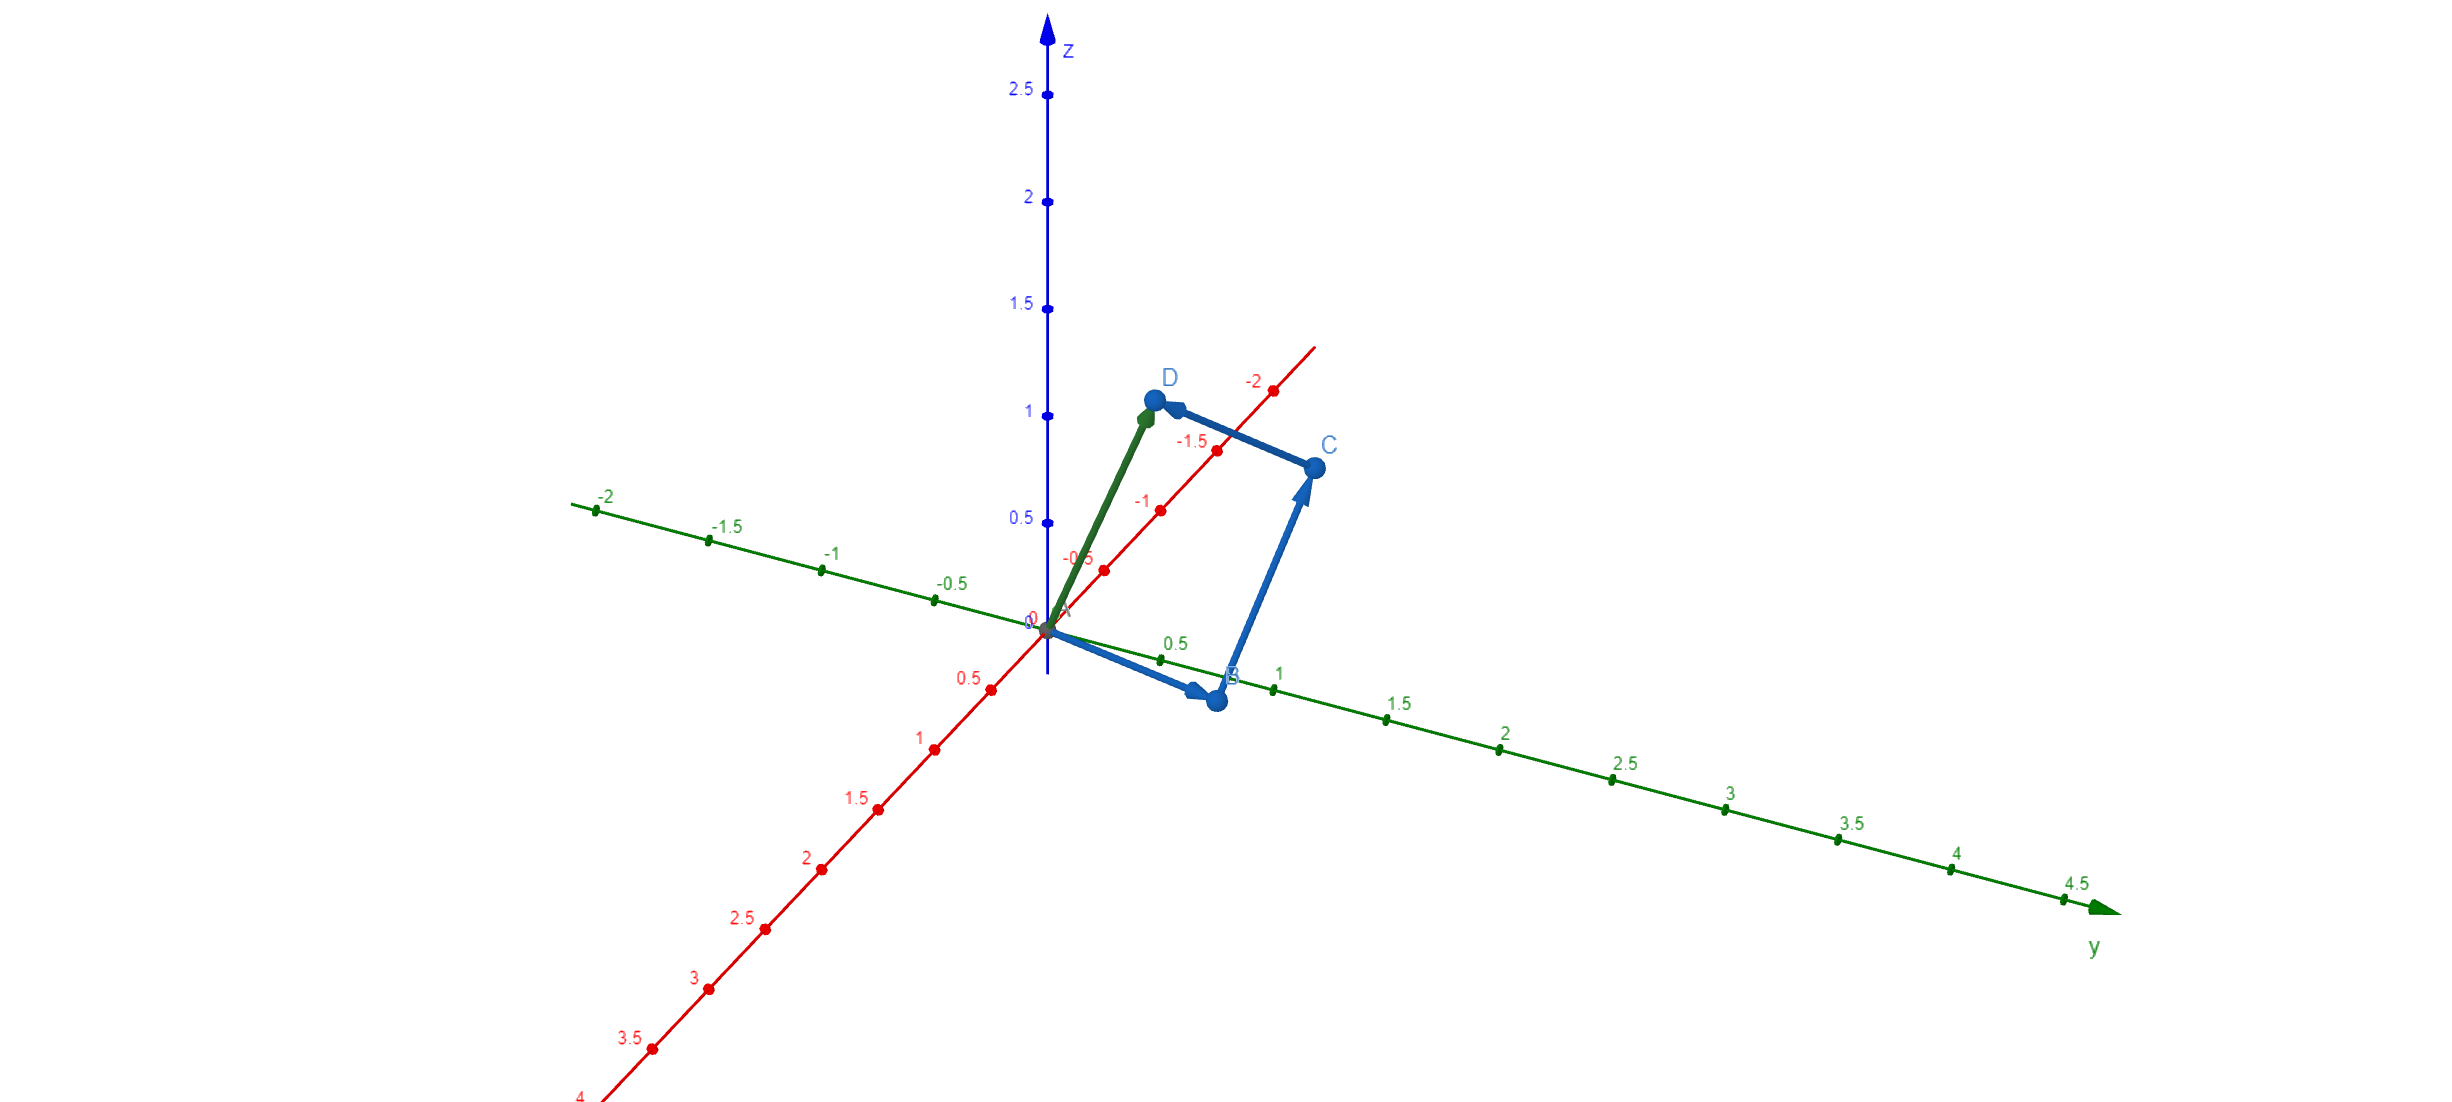
\includegraphics[height=200px]{4.4.png}
    
    
    
% evaluation paper
\newpage
\[
\renewcommand{\arraystretch}{2}
\begin{tabular}{| c | c |}
 \hline
    \hugeУчастник & \hugeВклад в \% \\
 \hline
    \hugeКаренин Константин & \huge33.(3) \\
 \hline
    \hugeГонин Сергей & \huge33.(3) \\
 \hline
    \hugeТемиров Тимур & \huge33.(3) \\
 \hline
\end{tabular}
\]
\end{document}